% !TeX root = ../main.tex

% \begin{frame}
%   \frametitle{Issues with the Geometric TCC}
%
%   \begin{textblock*}{12cm}(0.5cm,2cm)
%     \begin{small}
%       \begin{itemize}
%         \item Cannot compute the homology of offsets directly.
%         \item Do not know $\mathbf{dim}~\hom_0(D\setminus B_\omega)$.
%         \item Cannot compute the homology of complements directly.
%       \end{itemize}
%     \end{small}
%   \end{textblock*}
%
% \end{frame}

\begin{frame}
  \frametitle{Overview: Computing the TCC}

  \begin{textblock*}{11cm}(1cm,2cm)
    Unknown $c$-Lipschitz function $f : D\to \R$.\vspace{1ex}

    \only<2,3>{Finite sample $P\subset D$ of $f$.\vspace{1ex}}

    \only<3>{Pair of neighborhood graphs on $P$.}
  \end{textblock*}

  \begin{textblock*}{12cm}(0.5cm,4.5cm)
    \includegraphics<1>[trim=50 200 50 200, clip, width=0.45\textwidth]{figures/nbhd/D}%
    \includegraphics<2>[trim=50 200 50 200, clip, width=0.45\textwidth]{figures/nbhd/P}%
    \includegraphics<3>[trim=50 200 50 200, clip, width=0.45\textwidth]{figures/nbhd/NP0}%
    \includegraphics<3>[trim=50 200 50 200, clip, width=0.45\textwidth]{figures/nbhd/NP1}
  \end{textblock*}
\end{frame}

\begin{frame}
  \frametitle{Overview: Computing the TCC}

  \begin{textblock*}{11cm}(1cm,2cm)
    Sublevel set $B_\omega$ that \emph{surrounds} $D$.\vspace{1ex}

    \only<2,3>{Samples $Q_0, Q_1\subset P$ near $B_\omega$\vspace{1ex}}

    \only<3>{Rips tells us about $(P^\delta, Q_0^\delta)\hookrightarrow (P^\delta, Q_1^\delta)$}
  \end{textblock*}

  \begin{textblock*}{12cm}(0.5cm,4.5cm)
    \includegraphics<1>[trim=50 200 50 200, clip, width=0.45\textwidth]{figures/nbhd/B0}%
    \includegraphics<2>[trim=50 200 50 200, clip, width=0.45\textwidth]{figures/nbhd/NQ0}%
    \includegraphics<2>[trim=50 200 50 200, clip, width=0.45\textwidth]{figures/nbhd/NQ1}%
    \includegraphics<3>[trim=50 200 50 200, clip, width=0.45\textwidth]{figures/nbhd/PQ0}%
    \includegraphics<3>[trim=50 200 50 200, clip, width=0.45\textwidth]{figures/nbhd/PQ1}
  \end{textblock*}
\end{frame}


\begin{frame}
  \frametitle{{\small Assumption 2, Duality, and the Algorithmic TCC}}

  \begin{textblock*}{12cm}(0.5cm,2cm)
    \begin{small}
      \begin{itemize}
        \item Cannot compute the homology of offsets directly.
        \item Do not know $\mathbf{dim}~\hom_0(D\setminus B_\omega)$.
        \item Cannot compute the homology of complements directly.
      \end{itemize}
    \end{small}
  \end{textblock*}
\end{frame}

\begin{frame}
  \frametitle{{\small Assumption 2, Duality, and the Algorithmic TCC}}

  % \end{tikzcd}\end{equation}
  \begin{textblock*}{11cm}(1cm,2cm)
    \begin{small}
      Let $B_0 = B_{\omega-2c\delta}$\vspace{1ex}

      \only<2>{\begin{description}
        \item[Assumption 2] $\hom_0(D\setminus B_\omega\hookrightarrow D\setminus B_{0})$ is \emph{injective}.
      \end{description}}

      \only<3>{\begin{lemma}\label{lem:assumption2}
        If $\hom_0(D\setminus B_\omega\hookrightarrow D\setminus B_{0})$ is injective then $\mathbf{dim}~\hom_0(\rips^\delta(P\setminus Q_{0})) \geq \mathbf{dim}~\hom_0(D\setminus B_\omega)$.
      \end{lemma}}
    \end{small}
  \end{textblock*}

  \begin{textblock*}{12cm}(1cm,5.5cm)
    \includegraphics<2,3>[trim=300 200 200 200, clip, width=0.4\textwidth]{../scripts/figures/surf/ass2_C_top.png}\hspace{6ex}%
    \includegraphics<2,3>[trim=300 200 200 200, clip, width=0.4\textwidth]{../scripts/figures/surf/ass2_B_top.png}
  \end{textblock*}

  % \begin{textblock*}{12cm}(1cm,4.5cm)
  %   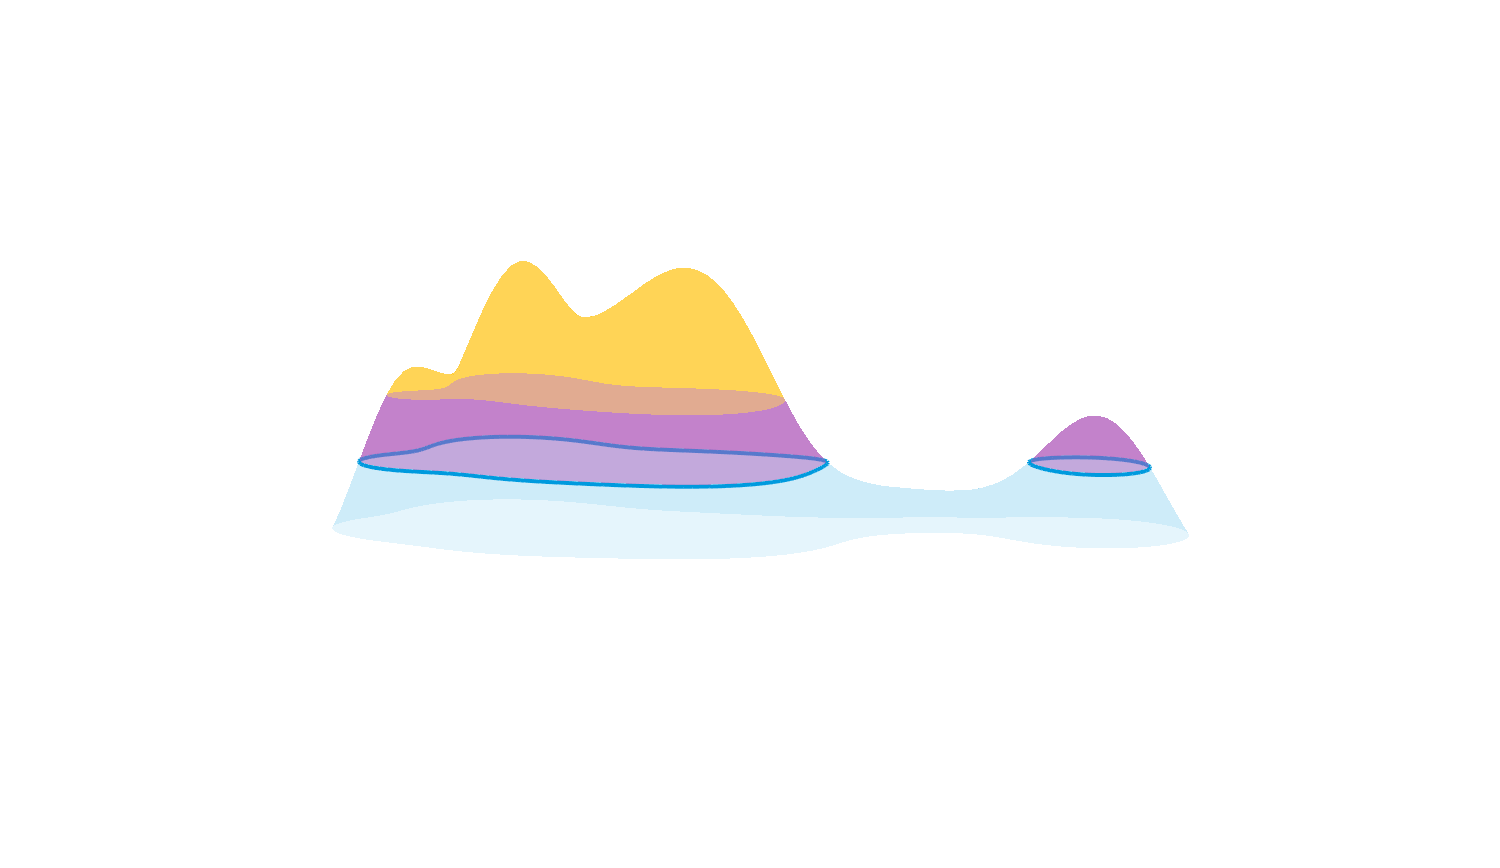
\includegraphics[trim=200 300 200 200, clip, width=0.5\textwidth]{../scripts/figures/surf/ass2_C_side.png}%
  %   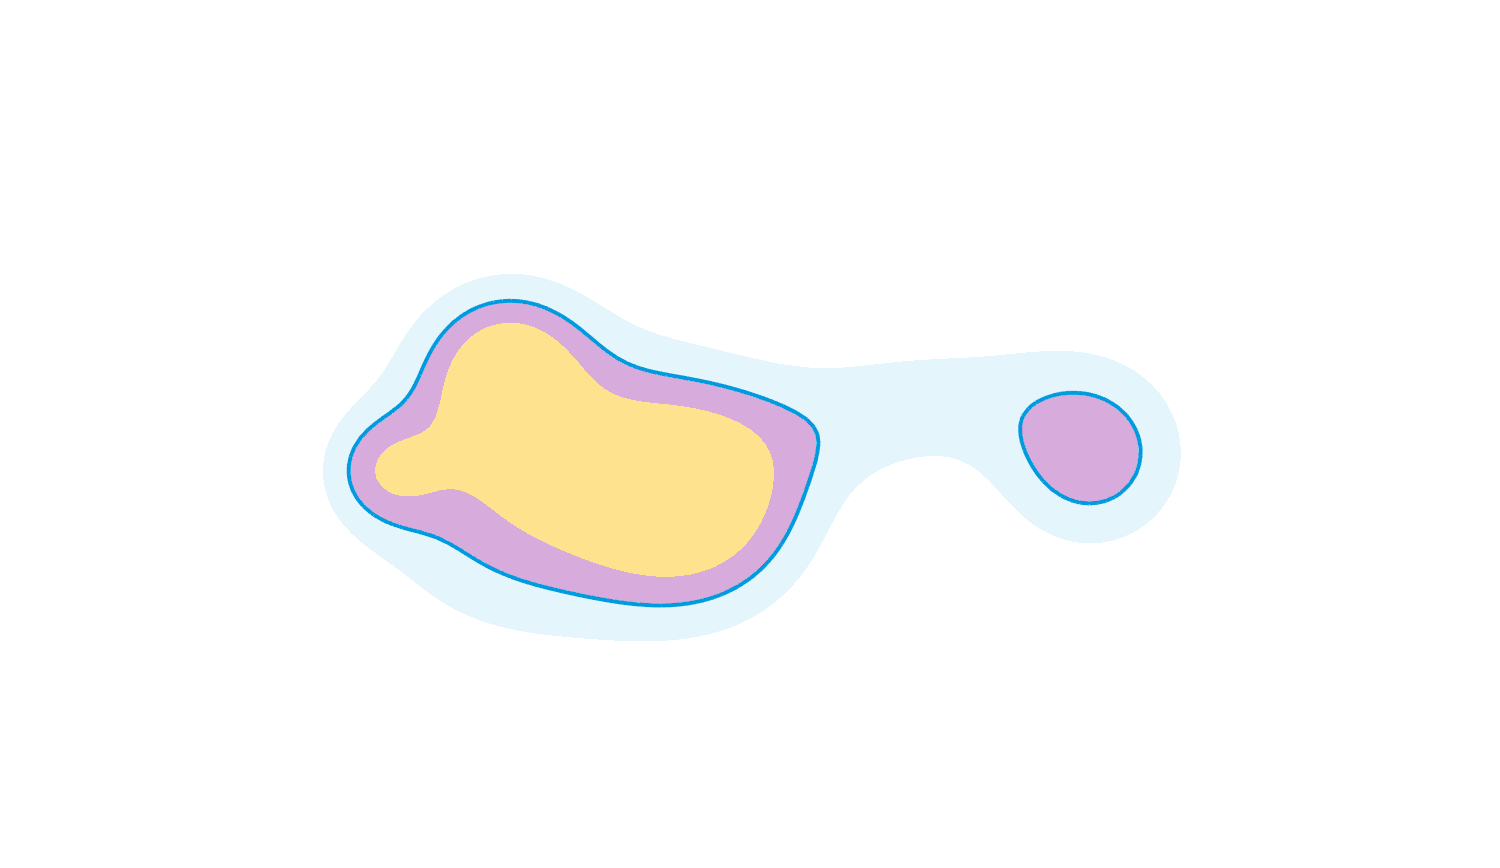
\includegraphics[trim=300 200 200 200, clip, width=0.3\textwidth]{../scripts/figures/surf/ass2_C_top.png}%
  %   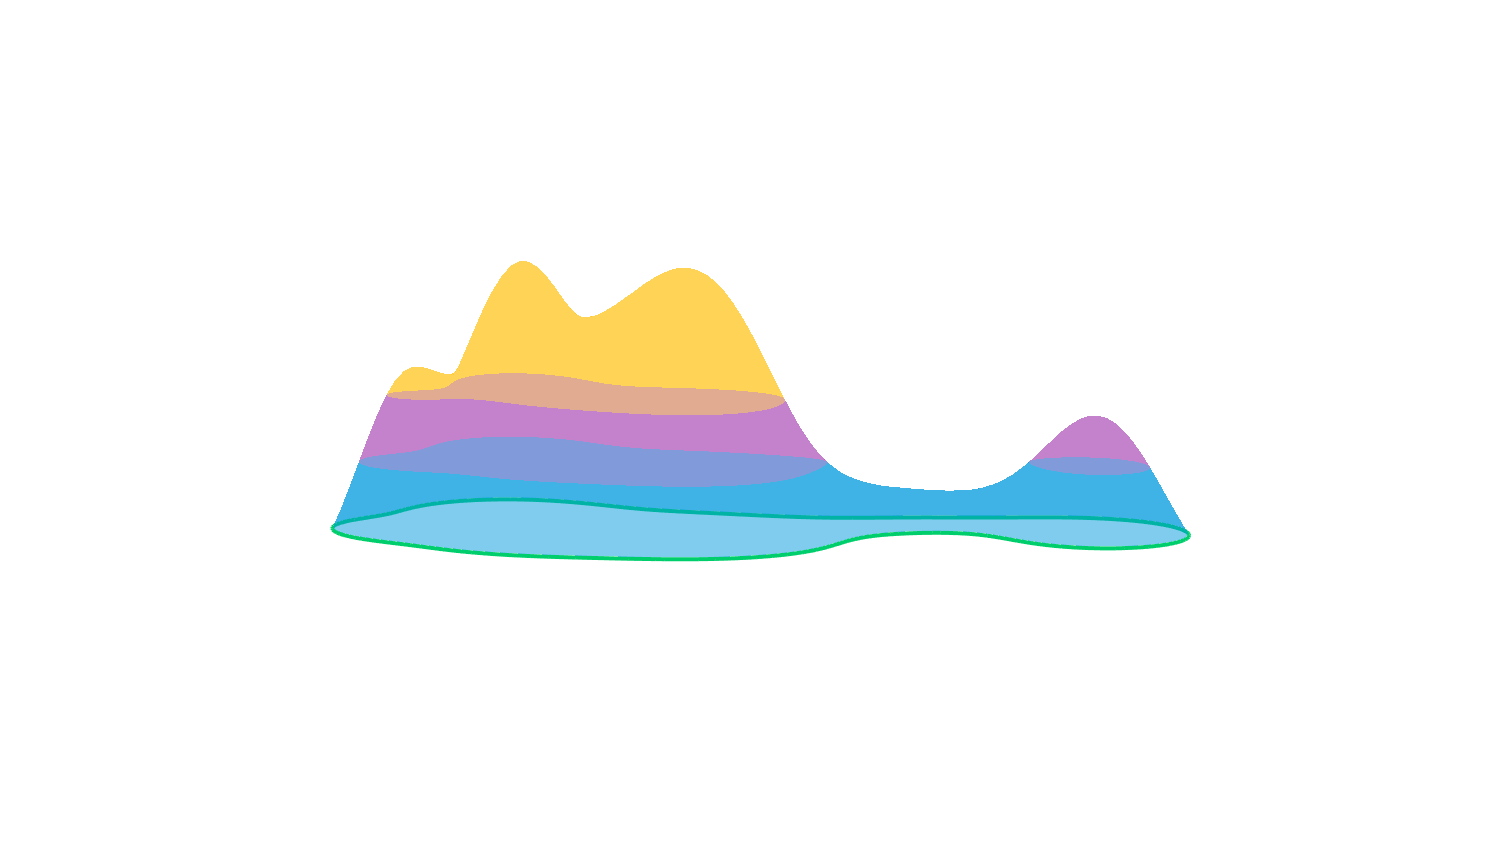
\includegraphics[trim=200 300 200 200, clip, width=0.5\textwidth]{../scripts/figures/surf/ass2_B_side.png}%
  %   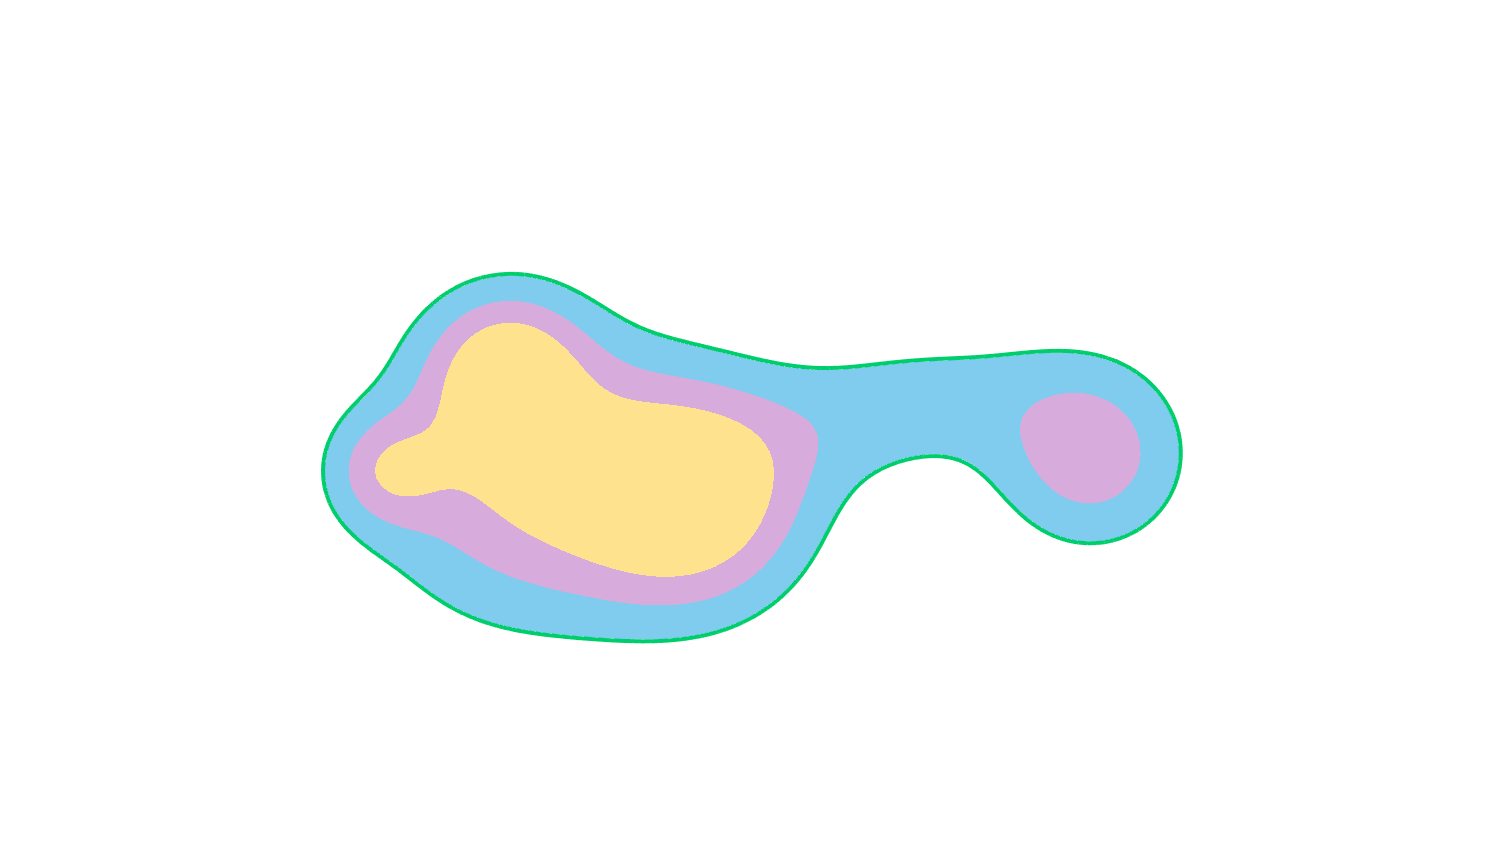
\includegraphics[trim=300 200 200 200, clip, width=0.3\textwidth]{../scripts/figures/surf/ass2_B_top.png}
  % \end{textblock*}
\end{frame}


\begin{frame}
  \frametitle{{\small Assumption 2, Duality, and the Algorithmic TCC}}

  \begin{textblock*}{12cm}(0.5cm,2cm)
    \begin{small}
      \begin{itemize}
        \item Cannot compute the homology of offsets directly.
        \item Do not know $\mathbf{dim}~\hom_0(D\setminus B_\omega)$.
        \item Cannot compute the homology of complements directly.
      \end{itemize}
    \end{small}
  \end{textblock*}
\end{frame}

\begin{frame}
  \frametitle{{\small Assumption 2, Duality, and the Algorithmic TCC}}

  \begin{textblock*}{11cm}(1cm,2cm)
    \begin{description}
      \item[Duality] $\hom_d(P^\e,Q^\e)\cong\hom_0(D\setminus Q^\e, D\setminus P^\e)$.
    \end{description}
  \end{textblock*}

  \begin{textblock*}{11cm}(1cm,5cm)
    \centering
    \includegraphics<2>[width=0.8\textwidth]{figures/balloons1}%
    \includegraphics<3>[width=0.8\textwidth]{figures/balloons2}%
    \includegraphics<4>[width=0.8\textwidth]{figures/balloons3}
  \end{textblock*}
\end{frame}

\begin{frame}
  \frametitle{{\small Assumption 2, Duality, and the Algorithmic TCC}}

  \begin{textblock*}{11cm}(1cm,2cm)
    \begin{small}\begin{theorem}[Algorithmic TCC]
        If
        \[ \mathbf{rk}~\hom_d(\rips^\delta(P,Q_0)\hookrightarrow \rips^{2\delta}(P, Q_1))\geq \mathbf{dim}~\hom_0(\rips^\delta(P\setminus Q_{0}))\]
        then $D\setminus B_\omega\subseteq P^\delta$ and $Q_0^\delta$ surrounds $P^\delta$ in $D$.
    \end{theorem}\end{small}
  \end{textblock*}
\end{frame}
